% Real-flight results chart for the A1 poster. Compile on its own, then in the poster:
%   \includegraphics[width=\linewidth]{images/fig_results_poster.pdf}
% Numbers: mean tracking error per phase from the flight logs (policy I1, 2026-11-04).
\documentclass[12pt, border=4pt]{standalone}
\usepackage{pgfplots}
\pgfplotsset{compat=1.18}
\renewcommand{\familydefault}{\sfdefault}

\definecolor{saclaydk}{RGB}{27,67,32}
\definecolor{mandarine}{RGB}{243,115,32}
\definecolor{vert}{RGB}{140,198,62}
\definecolor{bleu}{RGB}{80,144,205}
\definecolor{rouge}{RGB}{198,11,70}

\begin{document}
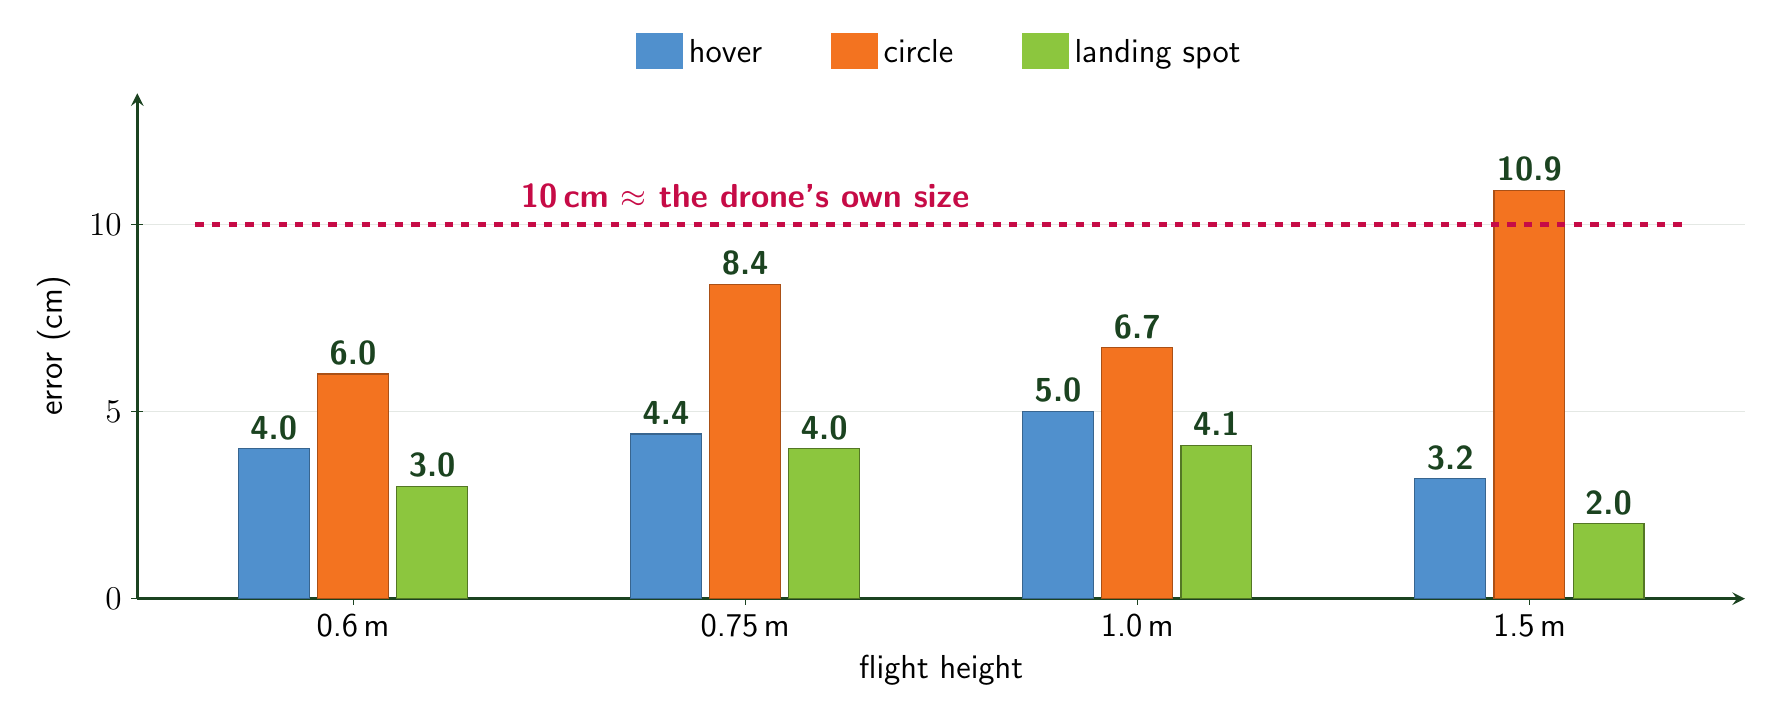
\begin{tikzpicture}
  \begin{axis}[
      width=22cm, height=8cm,
      ybar=3pt, bar width=0.9cm,
      ymin=0, ymax=13.5, ylabel={error (cm)},
      xmin=0.45, xmax=4.55,
      xtick={1,2,3,4}, xticklabels={0.6\,m, 0.75\,m, 1.0\,m, 1.5\,m},
      xlabel={flight height},
      axis lines=left, axis line style={saclaydk, line width=1pt}, tick style={saclaydk},
      ytick={0,5,10}, ymajorgrids, grid style={saclaydk!12},
      tick label style={font=\large}, label style={font=\large},
      nodes near coords={\pgfmathprintnumber[fixed, fixed zerofill, precision=1, assume math mode=true]{\pgfplotspointmeta}},
      nodes near coords style={font=\large\bfseries, text=saclaydk},
      legend style={at={(0.5,1.03)}, anchor=south, legend columns=3, draw=none,
                    font=\large, /tikz/every even column/.append style={column sep=0.8cm}},
      legend image code/.code={\draw[#1, draw=none] (0cm,-0.2cm) rectangle (0.6cm,0.25cm);},
    ]
    \addplot[fill=bleu, draw=bleu!70!black]           coordinates {(1,4.0) (2,4.4) (3,5.0) (4,3.2)};
    \addplot[fill=mandarine, draw=mandarine!70!black] coordinates {(1,6.0) (2,8.4) (3,6.7) (4,10.9)};
    \addplot[fill=vert, draw=vert!60!black]           coordinates {(1,3.0) (2,4.0) (3,4.1) (4,2.0)};
    \legend{hover, circle, landing spot}
    % size reference
    \draw[rouge, dashed, line width=1.6pt] ([xshift=-2cm]axis cs:1,10) -- ([xshift=2cm]axis cs:4,10);
    \node[anchor=south, font=\large\bfseries, text=rouge] at (axis cs:2,10.2)
         {10\,cm $\approx$ the drone's own size};
  \end{axis}
\end{tikzpicture}
\end{document}
